\recipe{Ellie’s Biscoff Millionaire’s Shortbread}
\label{recipe:biscoff_millionaires_shortbread}
\makes{8 portions}
\worktime{\SI{30} \minute}
\totaltime{\SI{60} \minute}
\source{Ellie}


\begin{ingredients}

\ingroup{For the Base}
\item 550g Biscoff Biscuts, finely crushed
\item 250g Butter (Melted)
\ingroup{Caramel}
\item 1 tin (397g) Condensed Milk
\item 90g unsalted Butter
\item 100g light brown sugar
\item 2 tsp salt
\item 1 tbsp golden syrup
\ingroup{Topping}
\item 250g White Chocolate
\item 100g Biscoff spread + 5g for the
swirl
\end{ingredients}


\begin{method}
  	Crush biscuits really small and mix with the melted butter 

Tip into a lined tin and press down to make an even base, then put
in fridge

Put all the caramel ingredients into a pan and bring to the  boil,
mixing all the time. Simmer until it forms soft balls when dropped
into cold water

Pour over the soft biscuit base and put it back in the fridge

Melt the white choc and biscoff spread together. Then pour over
the caramel.

Melt the extra biscoff spread and drizzle over the choclate in lines
Drag a knife through to marble

Put in the fridge until solid

Cut into pieces and enjoy
  
\end{method}


\begin{figure}[h]
  \centering
  
  \begin{minipage}{0.49\linewidth}
  	\centering
	\begin{tikzpicture}
  		% Save the image in a box to get its dimensions
  		\sbox0{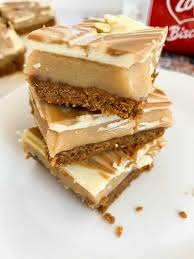
\includegraphics[width = \linewidth]{images/biscoffMillionaresShortbread.jpeg}}%
  
  		% Draw a clipping rectangle with rounded corners
  		\path[clip, rounded corners=0.5cm] (0,0) rectangle (\wd0,\ht0);
  
  		% Place the image inside the clipped area
  		\node[inner sep=0pt, outer sep=0pt, anchor=south west] at (0, 0) {\usebox0};
	\end{tikzpicture}
  \end{minipage}
  \hfill
  \begin{minipage}{0.49\linewidth}
  	\centering
	\begin{tikzpicture}
  		% Save the image in a box to get its dimensions
  		\sbox0{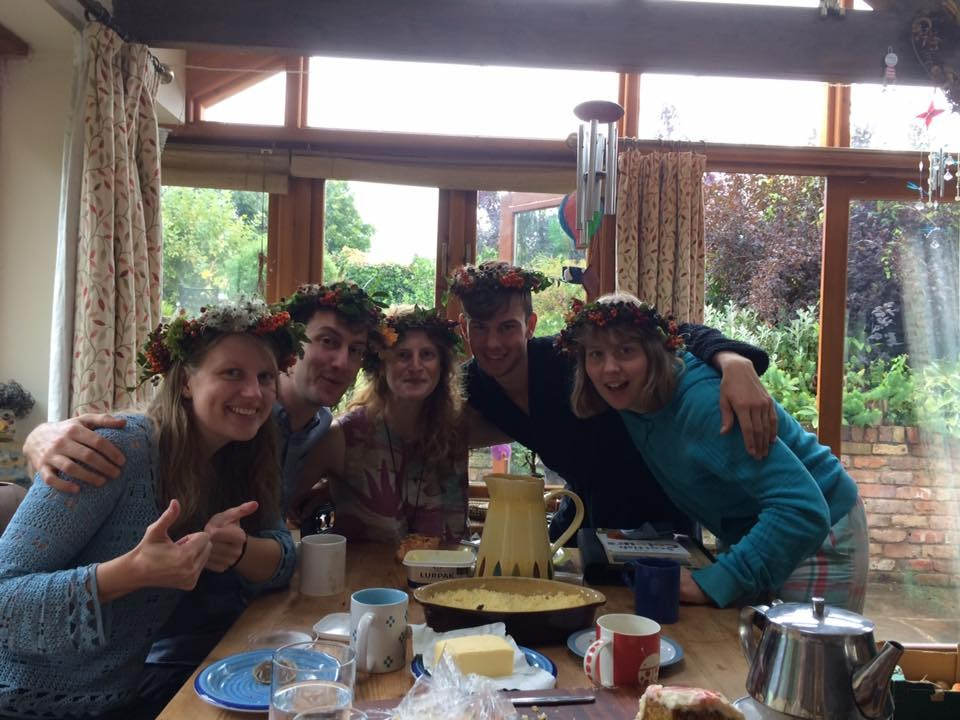
\includegraphics[width = \linewidth]{images/franFamily.jpeg}}%
  
  		% Draw a clipping rectangle with rounded corners
  		\path[clip, rounded corners=0.5cm] (0,0) rectangle (\wd0,\ht0);
  
  		% Place the image inside the clipped area
  		\node[inner sep=0pt, outer sep=0pt, anchor=south west] at (0, 0) {\usebox0};
	\end{tikzpicture}
  \end{minipage}
\end{figure}

